\renewcommand\paragraph{\@startsection{paragraph}{4}{\z@}%
                                     {-3.25ex\@plus -1ex \@minus -.2ex}%
                                     {0.0001pt \@plus .2ex}%
                                     {\normalfont\normalsize\bfseries}}

\renewcommand\subparagraph{\@startsection{subparagraph}{5}{\z@}%
                                     {-3.25ex\@plus -1ex \@minus -.2ex}%
                                     {0.0001pt \@plus .2ex}%
                                     {\normalfont\normalsize\bfseries}}

\section{Modelo del Experimento}

\subsection{Experimento}
El experimento ha de poner a prueba la red neuronal desarrollada ante la presencia de diferentes factores. En contraposici\'{o}n, mediante la colaboraci\'{o}n del Centro de Control de Tr\'{a}nsito del MOPT, se evaluar\'{a}n los mismos factores o eventos para obtener un resultado estimado de acuerdo con el sistema que actualmente emplean. De esta forma, se busca contrastar las respuestas obtenidas por el sistema, contra los resultados que genere la red neuronal bajo las mismas condiciones. Adicionalmente, interesa determinar si la red neuronal brinda una respuesta adecuada ante las diferentes combinaciones de eventos que se definen posteriormente y de esta forma establecer un punto de referencia de la eficiencia y factibilidad de poder realizar en un futuro una implementaci\'{o}n real. 

Cabe destacar que este experimento es de tipo multifactorial, por lo cual se han de evaluar las combinaciones de los diferentes factores que se presenten.

\subsection{Factores}
Bas\'{a}ndose en eventos y condiciones que tienden a presentarse en la mayor\'{i}a de zonas del pa\'{i}s, se determinaron los factores a ser tomados en cuenta para la realizaci\'{o}n de este experimento. Cada factor consta de dos a tres niveles a ser tomados en cuenta, dichos niveles corresponden a la dificultad que el evento conlleva para los otros veh\'{i}culos dentro de la zona. Los factores se explican a continuaci\'{o}n.


\subsection{Descripci\'{o}n de Factores}

En los siguientes apartados se describen la forma en que se han de realizar los diferentes factores a simular mediante el sistema utilizado en el Centro de Control de Tr\'{a}nsito.  Los mismos se encuentran ordenados seg\'{u}n el impacto y frecuencia con que estos se pueden presentar.

Adicionalmente, se tomar\'{a} como velocidad promedio para los veh\'{i}culos de 50km/h y ser\'{a}n ambientadas dentro de la zona comprendida por las \textbf{Avenidas:} 2, 4, 6 y 8 y las \textbf{Calles:} 6, 8, 10 y 12. Finalmente, la hora a emplear para las simulaciones corresponde a la hora pico de la tarde, desde las 4pm a las 6:30 pm aproximadamente.

\subsubsection{Accidentes de Tr\'{a}nsito}
Para la selecci\'{o}n de estos se tom\'{o} como base el mapa de distribuci\'{o}n espacial de accidentes para la zona obtenida del “Estudio de la distribuci\'{o}n espacial de accidentes de tr\'{a}nsito con v\'{i}ctimas en el cant\'{o}n de San Jos\'{e}” el cual fue proporcionado por el Consejo de Seguridad Vial. Para estos casos se utilizaron calles o avenidas de la zona que, de acuerdo con el estudio, presentan una mayor  concentraci\'{o}n de accidentes. El \'{a}rea correspondiente a la localizaci\'{o}n de cada accidente se muestra marcada con una zona blanca con borde negro dentro de cada mapa.

\subparagraph{Nivel 0}

Corresponde a: “Ausencia de accidentes”. Se evaluar\'{a} el caso en que no se presente accidentes de ning\'{u}n tipo dentro de la zona especificada.

\subparagraph{Nivel 1}

Corresponde a: “Choque entre dos veh\'{i}culos bloqueando un carril en el extremo final de la calle”.  La idea de este evento es que el accidente se ubique cerca del sem\'{a}foro correspondiente a la avenida y calle que se seleccionen, permitiendo de esta forma simular el caso en el cual los dem\'{a}s veh\'{i}culos puedan ocupar el espacio disponible en el tramo restante, previniendo que se presenten tantos problemas para los veh\'{i}culos que provengan de otras direcciones.

Dicho choque se ha de realizar en la Avenida 6 y 8 con la calle 8 tal y como se muestra en la figura \ref{fig:acc1}.

\begin{figure}[htp]
	\centering
	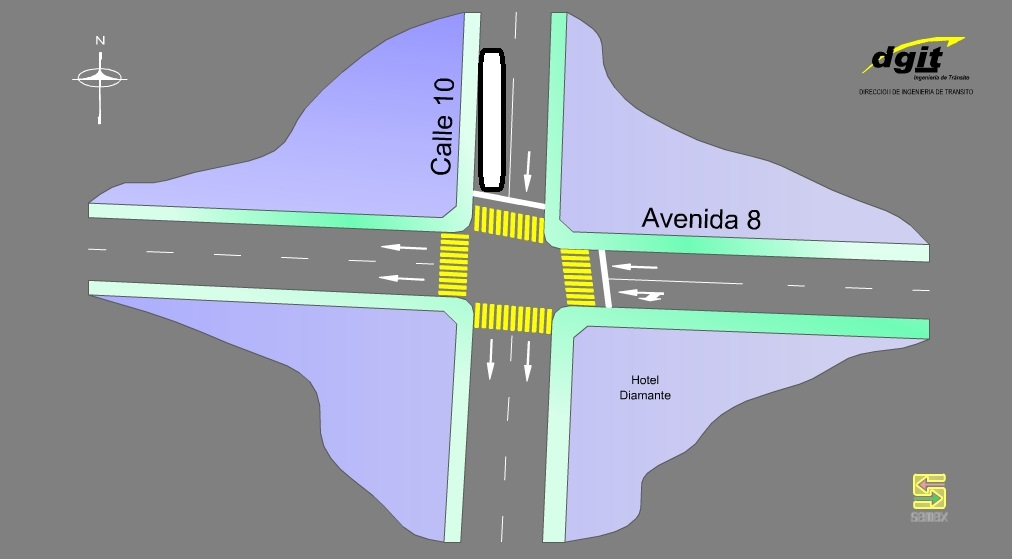
\includegraphics[scale=0.4]{images/117_AV08_CA10_Acc1.jpg}
	\caption{Accidente de Tr\'{a}nsito - Nivel 1}
	\label{fig:acc1}
\end{figure}

\subparagraph{Nivel 2}
Corresponde a: “Choque entre dos veh\'{i}culos bloqueando un carril en el extremo inicial de la calle”. El aumento de dificultad en este se debe a que el accidente ocurrir\'{a} justo despu\'{e}s de que hayan ingresado a la calle en cualquiera de los carriles, esto supone la dificultad de que los veh\'{i}culos localizados en calles adyacentes no contar\'{a}n con mucho espacio para ubicarse en una mejor posici\'{o}n que les permita continuar avanzando, lo que podr\'{i}a causar que muchos no avancen del sem\'{a}foro donde se encuentren en ese momento o que decidan tomar una ruta alterna.
Dicho choque se ha de realizar en la Avenida 6 con las calles 6 y 8 tal y como se muestra en la figura \ref{fig:acc2}.

\begin{figure}[H]
	\centering
	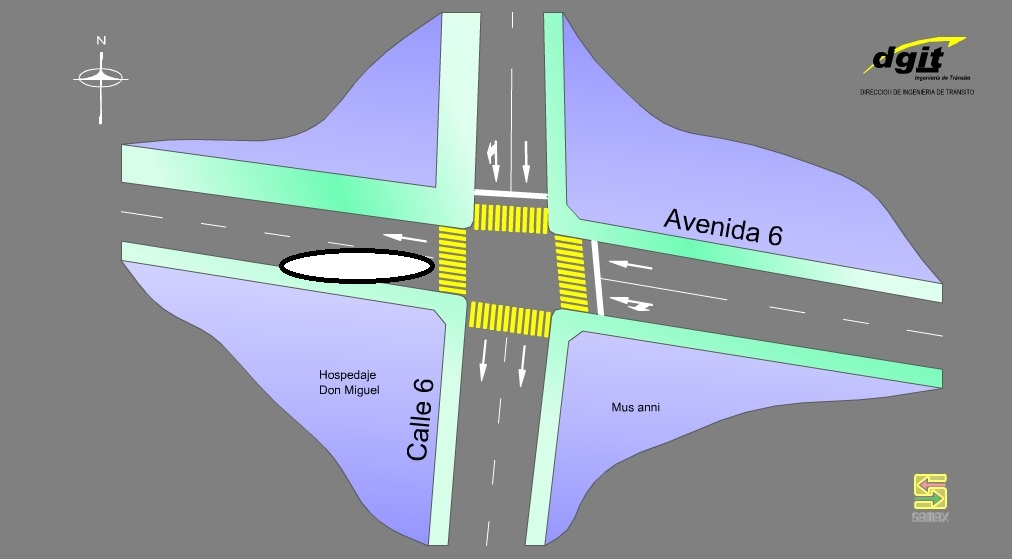
\includegraphics[scale=0.40]{images/145_AV06_CA06_Acc2.jpg}
	\caption{Accidente de Tr\'{a}nsito - Nivel 2}
	\label{fig:acc2}
\end{figure}

\subsubsection{Zonas de parqueo}
La idea de este  factor corresponde a un hecho caracter\'{i}stico como lo son paradas de autobuses, zonas de descarga y terminales en las calles. Si se analiza considerando que las calles posean un m\'{a}ximo de 2 carriles se pueden notar los siguientes comportamientos: si se poseen terminarles de buses, se habla de un carril pr\'{a}cticamente dedicado a estas, mientras que para el otro caso se poseen bloqueos temporales de un carril en ciertos puntos por un tiempo determinado como resultado de que los buses realicen paradas para subir o bajar pasajeros. 

Cabe mencionar que para este caso s\'{o}lo se consideran dos niveles para los factores por el hecho de realizar evaluaciones de otros resulta bastante dif\'{i}cil debido al grado de variaci\'{o}n que se presenta, tal es el caso de el parqueo temporal de veh\'{i}culos el cual depender\'{a} de cada persona, seg\'{u}n las habilidades y experiencia con las que cuenten para tardar m\'{a}s o menos tiempo en estacionar un veh\'{i}culo. 

\subparagraph{Nivel 0}

Corresponde a: “Ausencia de zonas de parqueo o paradas”. Se evaluar\'{a} el caso en que no se presente ninguna zona de parqueo o paradas, implicando que todas las calles de la zona se encuentran completamente dedicadas al tr\'{a}nsito de veh\'{i}culos.

\subparagraph{Nivel 1}

Corresponde a: “Parqueos para veh\'{i}culos, ocupar\'{a}n todo un carril, junto con este se tomar\'{a} en cuenta las paradas terminales de autobuses, son paradas fijas que siempre cuentan con autobuses en estas y abarcan un carril completo de la calle”. Se consideran carriles completos para alojar paradas o parqueos los cuales han de encontrarse ocupados en todo momento durante las evaluaciones, por lo que las calles pasar\'{a}n de contar con s\'{o}lo un carril disponible para que el resto de veh\'{i}culos transiten.

Las paradas a ser consideradas como permanentes corresponden a aquellas donde por lo general hay un bus subiendo pasajeros y otro esperando a salir, o en otros casos que apenas llega un nuevo bus el que estaba esperando parte de la parada. \'{e}stas son:\newline

\begin{table}[tb!hp]
	\centering
	\begin{tabular}{|c|c|c|}
		\hline
			\textbf{Avenidas} & \textbf{Calles} & \textbf{Cantidad Paradas}\\
		\hline
			2 & 12 a 10 & 3\\
		\hline
			2 & 10 a 8 & 1 (parada taxis)\\
		\hline
			2 & 8 a 6 & 3\\
		\hline
			2 a 4 & 6 & 1 (zona de descarga)\\
		\hline
			2 a 4 & 8 & 4\\
		\hline
			2 a 4 & 10 & 2\\
		\hline
			6 & 10 - 8 & 3\\
	\hline
	\end{tabular}

	\caption{Paradas permanentes San Jos\'{e}, Costa Rica}
	\label{tab:stops}
\end{table}

Las siguientes figuras muestran dichas zonas marcadas con un \'{a}rea (\'{o}valo blanco y negro) o con la leyenda “Parada de autob\'{u}s”. Cabe mencionar que a excepci\'{o}n de la figura correspondiente a parada de taxis, las dem\'{a}s representan paradas que se localizan a lo largo de la calle correspondiente.

\begin{figure}[H]
	\centering
	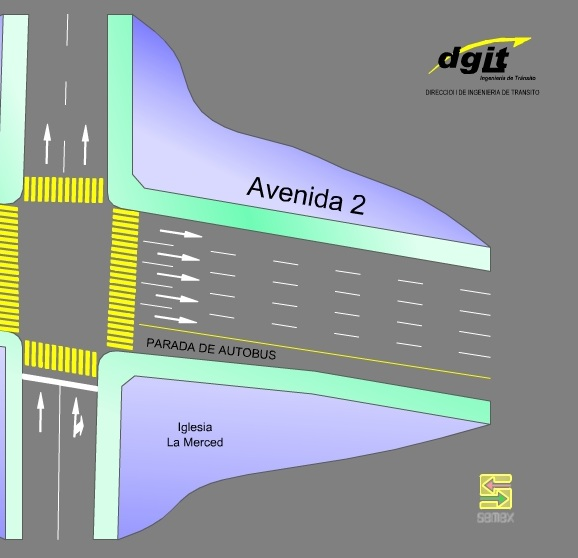
\includegraphics[width=14.2cm,height=8cm]{images/Parada_A2Ca12-10.jpg}
	\caption{Parada de autob\'{u}s Avenida 2, Calle 12 y 10}
	\label{fig:stopAv2Ca1210}
\end{figure}

\begin{figure}[H]
	\centering
	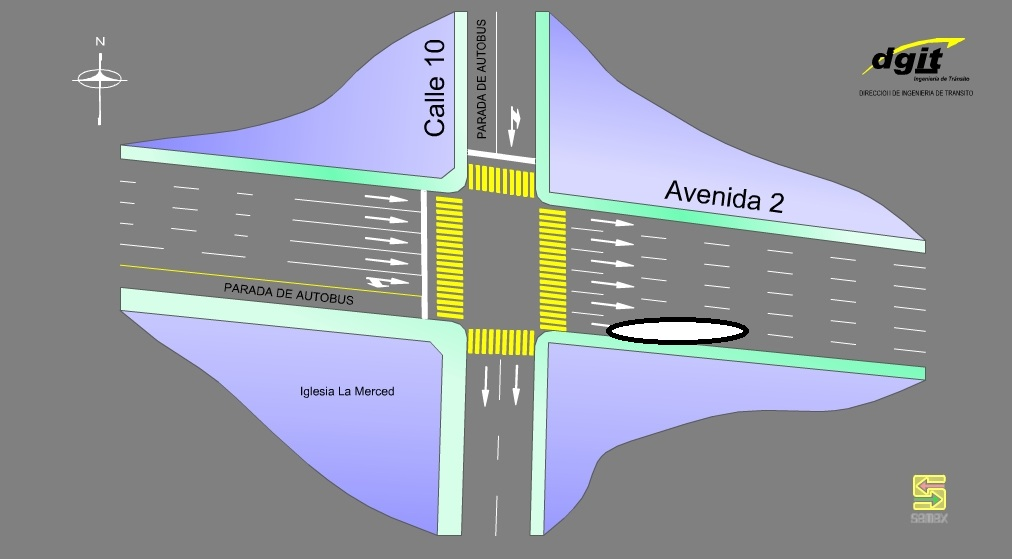
\includegraphics[scale=0.4]{images/Parada_A2Ca10-08.jpg}
	\caption{Parada de autob\'{u}s Avenida 2, Calle 12 y 10. Parada de taxis (\'{o}valo blanco) Avenida 2, Calle 10 y 8}
	\label{fig:stopAv2Ca1008}
\end{figure}

\begin{figure}[H]
	\centering
	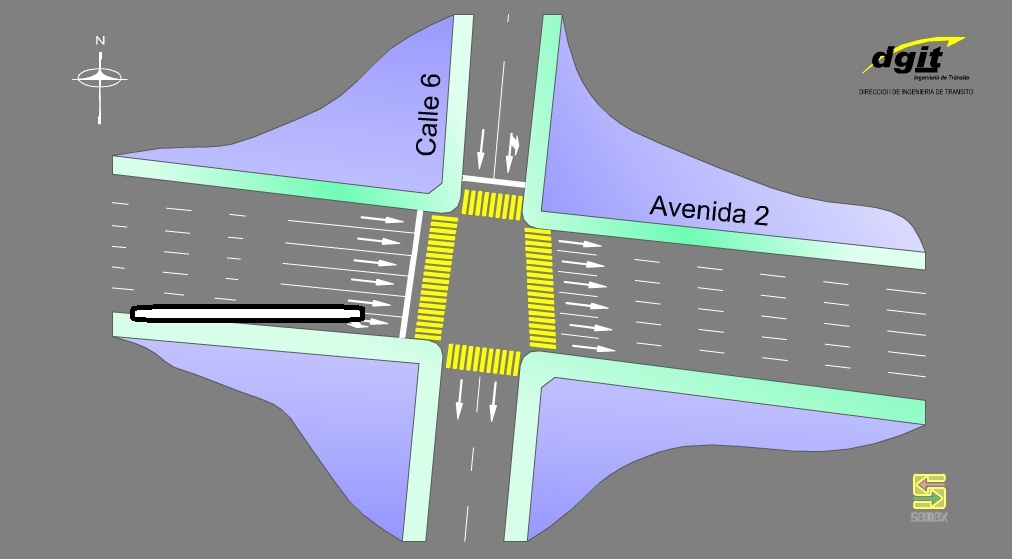
\includegraphics[scale=0.40]{images/Parada_A2Ca8-6.jpg}
	\caption{Parada de autob\'{u}s Avenida 2, Calle 6 y 8 (Hatillo)}
	\label{fig:stopAv2Ca0806}
\end{figure}

\begin{figure}[H]
	\centering
	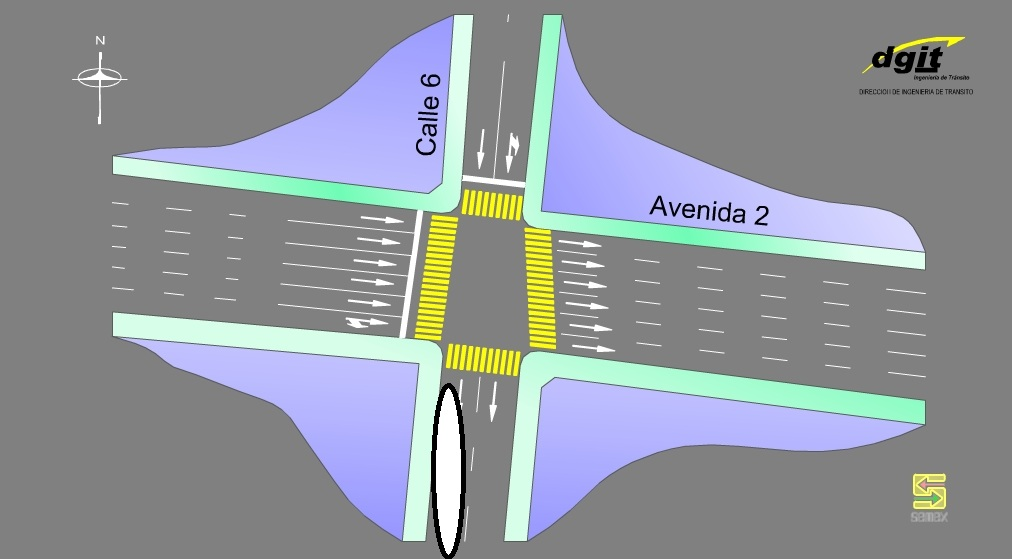
\includegraphics[scale=0.40]{images/Parada_A2-04Ca06.jpg}
	\caption{Zona de carga y descarga Avenida 2-4, Calle 6 (completo)}
	\label{fig:stopAv0204Ca6}
\end{figure}

\begin{figure}[H]
	\centering
	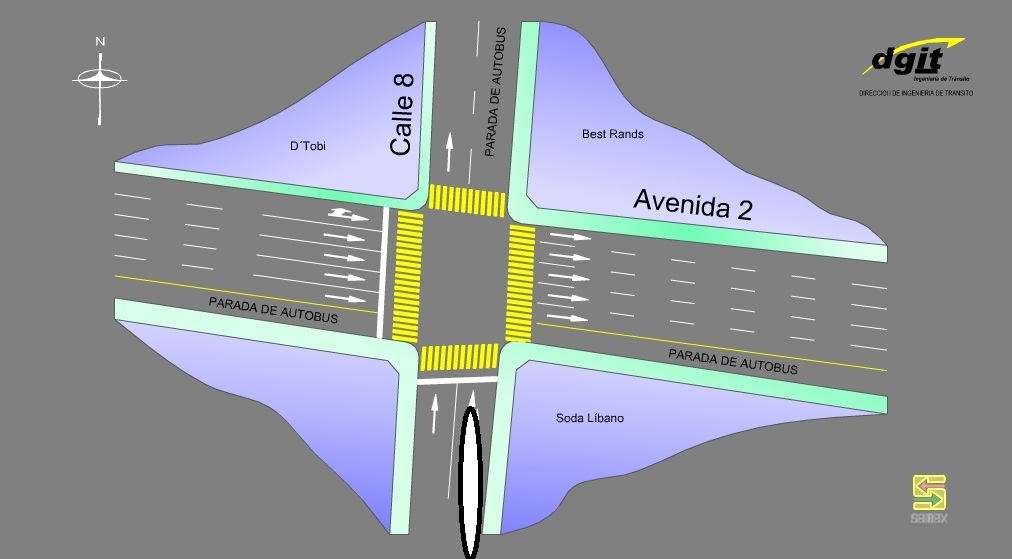
\includegraphics[scale=0.40]{images/Parada_A2-04Ca08.jpg}
	\caption{Parada de autob\'{u}s Avenida 2-4, Calle 8 (Completo)}
	\label{fig:stopAv0204Ca8}
\end{figure}

\begin{figure}[H]
	\centering
	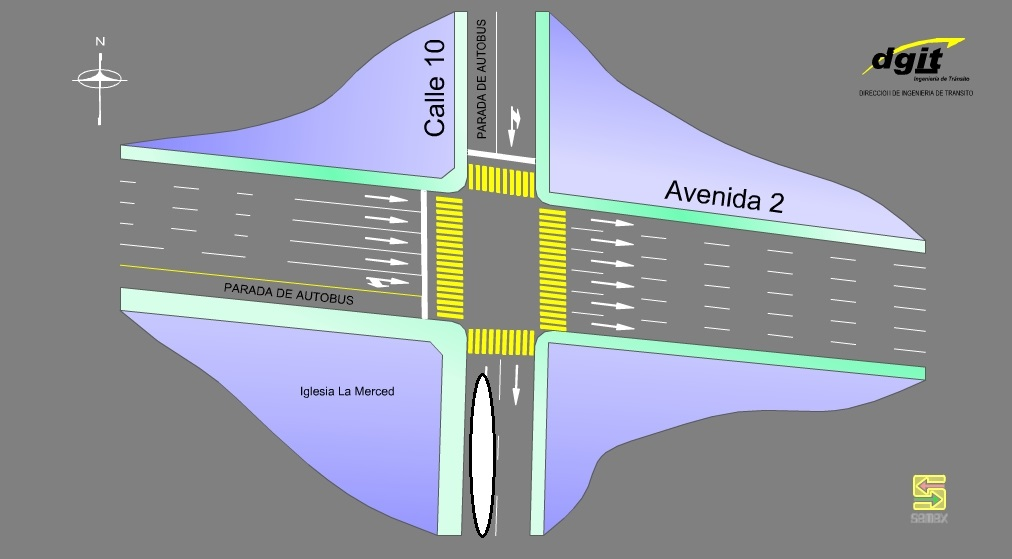
\includegraphics[scale=0.40]{images/Parada_A2-04Ca10.jpg}
	\caption{Parada de autob\'{u}s Avenida 2-4, Calle 10}
	\label{fig:stopAv0204Ca10}
\end{figure}

\begin{figure}[H]
	\centering
	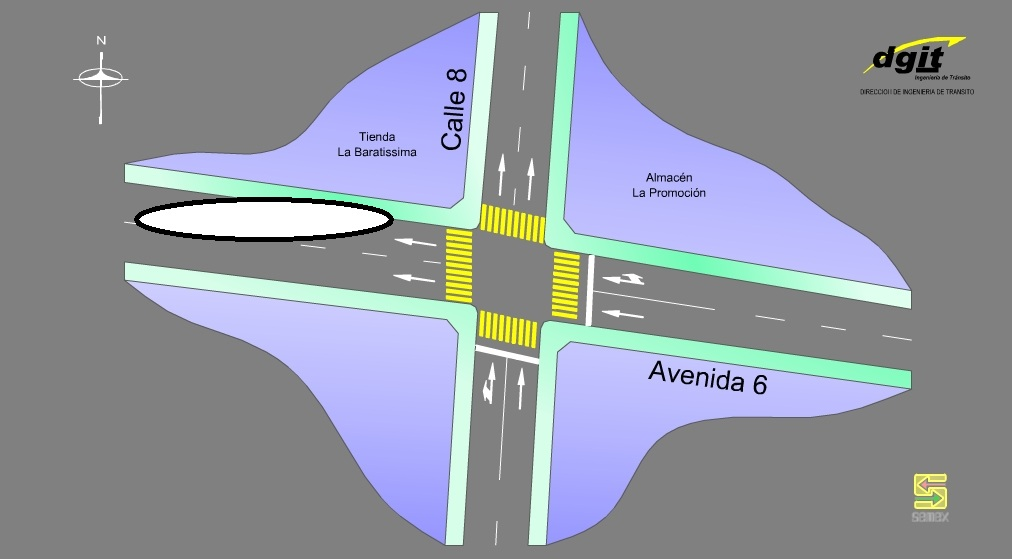
\includegraphics[scale=0.40]{images/Parada_A6Ca10-8.jpg}
	\caption{Parada de autob\'{u}s Avenida 6, Calle 10 y 8}
	\label{fig:stopAv6Ca1008}
\end{figure}

\subsubsection{Eventos meteorol\'{o}gicos}
Este factor var\'{i}a mucho pero igual se encuentra presente dentro de los factores que afectan y resulta necesario ser considerado. Para este caso, la presencia de lluvia en San Jos\'{e} ser\'{a} el principal circunstancia a evaluar tomando como punto de partida el hecho de que al presentarse los conductores tienden a reducir la velocidad con el fin de evitar accidentes por las dificultades para manejar que se presentan con la calle mojada o la poca visibilidad en caso de una lluvia fuerte.

Para este evento la velocidad promedio esperada es de 50km/h.

\subparagraph{Nivel 0}

Corresponde a: “Ausencia de lluvia en las calles”. Se evaluar\'{a} el caso en que no se presente lluvia por completo implicando que se mantenga la velocidad promedio mencionada anteriormente.

\subparagraph{Nivel 1}

Corresponde a: “Lluvia moderada dificultando la visibilidad y causando que los veh\'{i}culos reduzcan la velocidad”. Para este tipo de evento se considera una reducci\'{o}n m\'{a}s pronunciada bajando hasta los 30km/h.

\subsection{Combinaciones de factores (Escenarios)}
Como se pudo observar anteriormente, se poseen 3 factores de los cuales 2 cuentan con 2 niveles y el otro con 3 niveles. Por lo que se cuentan con 12 combinaciones, de esta forma la combinaci\'{o}n de los factores se muestra en la tabla \ref{tab:combFact} \bigskip


\begin{table}[tb!hp]
	\begin{tabular}{|c|c|c|c|}
	\hline
		& \multicolumn{1}{m{4.5cm}|}{\centering\textbf{Presencia de accidentes de tr\'{a}fico}} 
		 & \multicolumn{1}{m{4cm}|}{\centering\textbf{Zonas de Parqueo}} & 			\multicolumn{1}{m{4.5cm}|}{\textbf{Eventos Meteorol\'{o}gicos (lluvia)}}\\
	\hline
		1 & Nivel 0 & Nivel 0 & Nivel 0\\
	\hline
		2 & Nivel 1 & Nivel 0 & Nivel 0\\
	\hline
		3 & Nivel 2 & Nivel 0 & Nivel 0\\
	\hline
		4 & Nivel 0 & Nivel 1 & Nivel 0\\
	\hline
		5 & Nivel 1 & Nivel 1 & Nivel 0\\
	\hline
		6 & Nivel 2 & Nivel 1 & Nivel 0\\
	\hline
		7 & Nivel 0 & Nivel 0 & Nivel 1\\
	\hline
		8 & Nivel 1 & Nivel 0 & Nivel 1\\
	\hline
		9 & Nivel 2 & Nivel 0 & Nivel 1\\
	\hline
		10 & Nivel 0 & Nivel 1 & Nivel 1\\
	\hline
		11 & Nivel 1 & Nivel 1 & Nivel 1\\
	\hline
		12 & Nivel 2 & Nivel 1 & Nivel 1\\
	\hline
	\end{tabular}
	\caption{Combionaci\'{o}n de Factores}
	\label{tab:combFact}
\end{table}

